\begin{figure}[H]
    \begin{subfigure}{\textwidth}
        \centering
        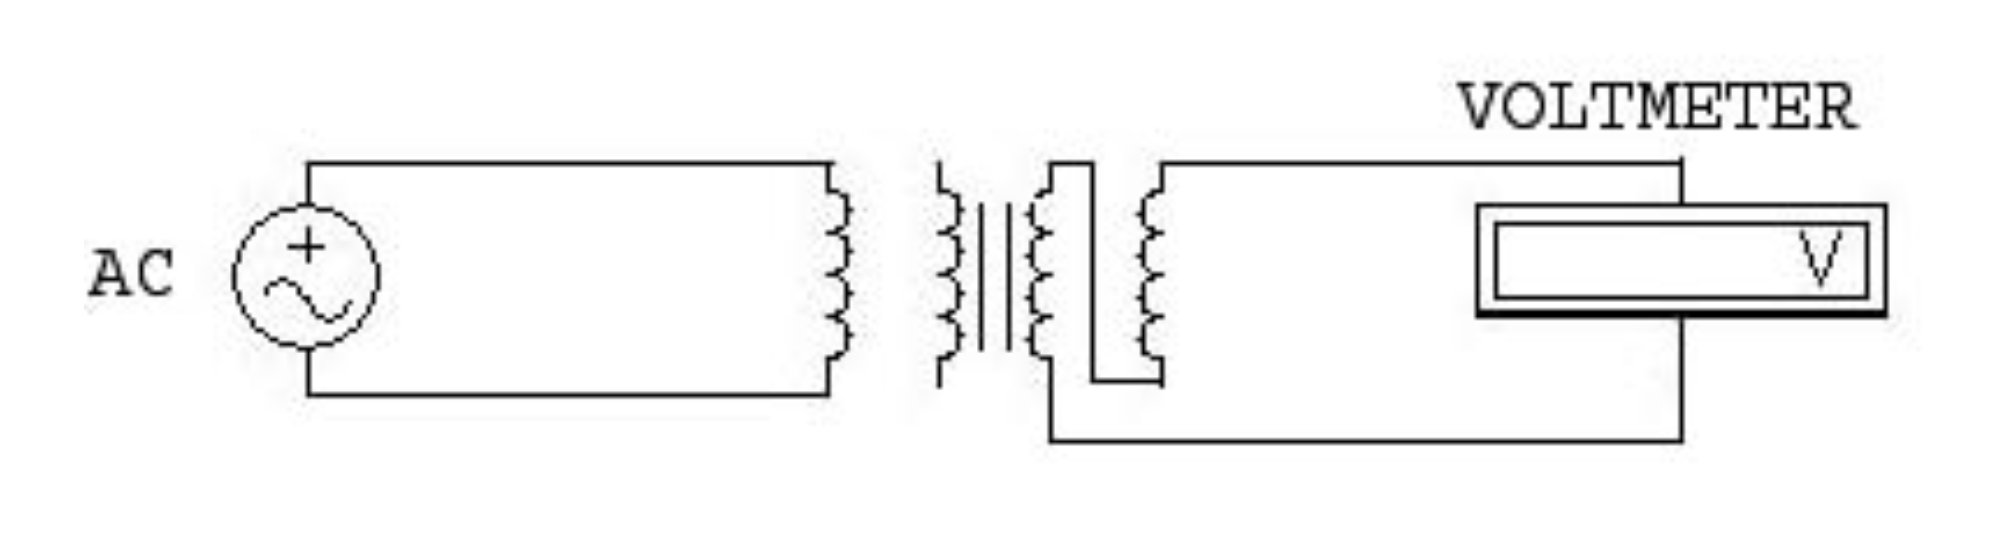
\includegraphics[width=.8\linewidth]{images/output/add.png}
        \caption{Additive (step-up) polarity.}
        \label{fig:sfig1}
    \end{subfigure}
    \begin{subfigure}{\textwidth}
        \centering
        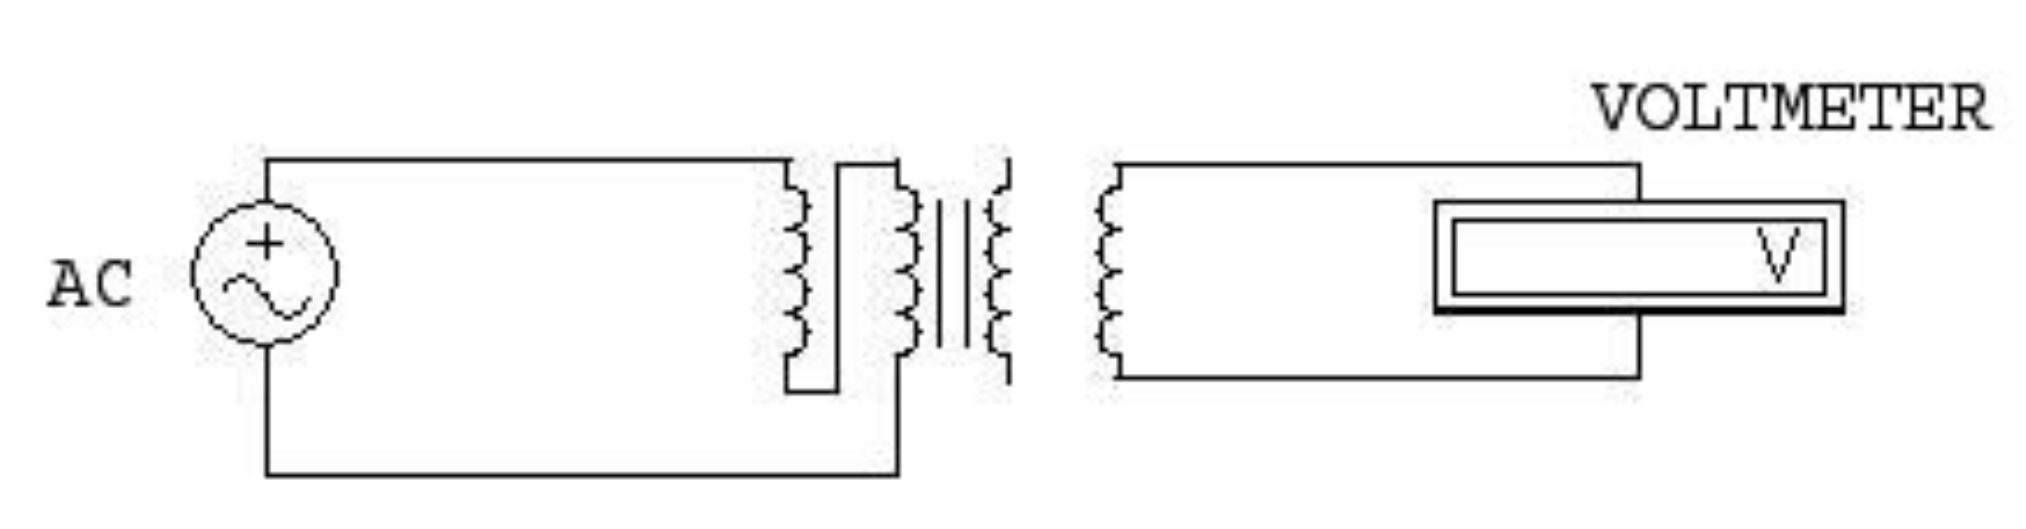
\includegraphics[width=.8\linewidth]{images/output/sub.png}
        \caption{Subtractive (step-down) polarity.}
        \label{fig:sfig2}
    \end{subfigure}
    \caption{Circuit diagrams for polarity test of transformer windings.}
    \label{fig:fig}
\end{figure}